% Options for packages loaded elsewhere
\PassOptionsToPackage{unicode}{hyperref}
\PassOptionsToPackage{hyphens}{url}
%
\documentclass[
]{article}
\usepackage{amsmath,amssymb}
\usepackage{lmodern}
\usepackage{iftex}
\ifPDFTeX
  \usepackage[T1]{fontenc}
  \usepackage[utf8]{inputenc}
  \usepackage{textcomp} % provide euro and other symbols
\else % if luatex or xetex
  \usepackage{unicode-math}
  \defaultfontfeatures{Scale=MatchLowercase}
  \defaultfontfeatures[\rmfamily]{Ligatures=TeX,Scale=1}
\fi
% Use upquote if available, for straight quotes in verbatim environments
\IfFileExists{upquote.sty}{\usepackage{upquote}}{}
\IfFileExists{microtype.sty}{% use microtype if available
  \usepackage[]{microtype}
  \UseMicrotypeSet[protrusion]{basicmath} % disable protrusion for tt fonts
}{}
\makeatletter
\@ifundefined{KOMAClassName}{% if non-KOMA class
  \IfFileExists{parskip.sty}{%
    \usepackage{parskip}
  }{% else
    \setlength{\parindent}{0pt}
    \setlength{\parskip}{6pt plus 2pt minus 1pt}}
}{% if KOMA class
  \KOMAoptions{parskip=half}}
\makeatother
\usepackage{xcolor}
\usepackage[margin=1in]{geometry}
\usepackage{color}
\usepackage{fancyvrb}
\newcommand{\VerbBar}{|}
\newcommand{\VERB}{\Verb[commandchars=\\\{\}]}
\DefineVerbatimEnvironment{Highlighting}{Verbatim}{commandchars=\\\{\}}
% Add ',fontsize=\small' for more characters per line
\usepackage{framed}
\definecolor{shadecolor}{RGB}{248,248,248}
\newenvironment{Shaded}{\begin{snugshade}}{\end{snugshade}}
\newcommand{\AlertTok}[1]{\textcolor[rgb]{0.94,0.16,0.16}{#1}}
\newcommand{\AnnotationTok}[1]{\textcolor[rgb]{0.56,0.35,0.01}{\textbf{\textit{#1}}}}
\newcommand{\AttributeTok}[1]{\textcolor[rgb]{0.77,0.63,0.00}{#1}}
\newcommand{\BaseNTok}[1]{\textcolor[rgb]{0.00,0.00,0.81}{#1}}
\newcommand{\BuiltInTok}[1]{#1}
\newcommand{\CharTok}[1]{\textcolor[rgb]{0.31,0.60,0.02}{#1}}
\newcommand{\CommentTok}[1]{\textcolor[rgb]{0.56,0.35,0.01}{\textit{#1}}}
\newcommand{\CommentVarTok}[1]{\textcolor[rgb]{0.56,0.35,0.01}{\textbf{\textit{#1}}}}
\newcommand{\ConstantTok}[1]{\textcolor[rgb]{0.00,0.00,0.00}{#1}}
\newcommand{\ControlFlowTok}[1]{\textcolor[rgb]{0.13,0.29,0.53}{\textbf{#1}}}
\newcommand{\DataTypeTok}[1]{\textcolor[rgb]{0.13,0.29,0.53}{#1}}
\newcommand{\DecValTok}[1]{\textcolor[rgb]{0.00,0.00,0.81}{#1}}
\newcommand{\DocumentationTok}[1]{\textcolor[rgb]{0.56,0.35,0.01}{\textbf{\textit{#1}}}}
\newcommand{\ErrorTok}[1]{\textcolor[rgb]{0.64,0.00,0.00}{\textbf{#1}}}
\newcommand{\ExtensionTok}[1]{#1}
\newcommand{\FloatTok}[1]{\textcolor[rgb]{0.00,0.00,0.81}{#1}}
\newcommand{\FunctionTok}[1]{\textcolor[rgb]{0.00,0.00,0.00}{#1}}
\newcommand{\ImportTok}[1]{#1}
\newcommand{\InformationTok}[1]{\textcolor[rgb]{0.56,0.35,0.01}{\textbf{\textit{#1}}}}
\newcommand{\KeywordTok}[1]{\textcolor[rgb]{0.13,0.29,0.53}{\textbf{#1}}}
\newcommand{\NormalTok}[1]{#1}
\newcommand{\OperatorTok}[1]{\textcolor[rgb]{0.81,0.36,0.00}{\textbf{#1}}}
\newcommand{\OtherTok}[1]{\textcolor[rgb]{0.56,0.35,0.01}{#1}}
\newcommand{\PreprocessorTok}[1]{\textcolor[rgb]{0.56,0.35,0.01}{\textit{#1}}}
\newcommand{\RegionMarkerTok}[1]{#1}
\newcommand{\SpecialCharTok}[1]{\textcolor[rgb]{0.00,0.00,0.00}{#1}}
\newcommand{\SpecialStringTok}[1]{\textcolor[rgb]{0.31,0.60,0.02}{#1}}
\newcommand{\StringTok}[1]{\textcolor[rgb]{0.31,0.60,0.02}{#1}}
\newcommand{\VariableTok}[1]{\textcolor[rgb]{0.00,0.00,0.00}{#1}}
\newcommand{\VerbatimStringTok}[1]{\textcolor[rgb]{0.31,0.60,0.02}{#1}}
\newcommand{\WarningTok}[1]{\textcolor[rgb]{0.56,0.35,0.01}{\textbf{\textit{#1}}}}
\usepackage{longtable,booktabs,array}
\usepackage{calc} % for calculating minipage widths
% Correct order of tables after \paragraph or \subparagraph
\usepackage{etoolbox}
\makeatletter
\patchcmd\longtable{\par}{\if@noskipsec\mbox{}\fi\par}{}{}
\makeatother
% Allow footnotes in longtable head/foot
\IfFileExists{footnotehyper.sty}{\usepackage{footnotehyper}}{\usepackage{footnote}}
\makesavenoteenv{longtable}
\usepackage{graphicx}
\makeatletter
\def\maxwidth{\ifdim\Gin@nat@width>\linewidth\linewidth\else\Gin@nat@width\fi}
\def\maxheight{\ifdim\Gin@nat@height>\textheight\textheight\else\Gin@nat@height\fi}
\makeatother
% Scale images if necessary, so that they will not overflow the page
% margins by default, and it is still possible to overwrite the defaults
% using explicit options in \includegraphics[width, height, ...]{}
\setkeys{Gin}{width=\maxwidth,height=\maxheight,keepaspectratio}
% Set default figure placement to htbp
\makeatletter
\def\fps@figure{htbp}
\makeatother
\setlength{\emergencystretch}{3em} % prevent overfull lines
\providecommand{\tightlist}{%
  \setlength{\itemsep}{0pt}\setlength{\parskip}{0pt}}
\setcounter{secnumdepth}{-\maxdimen} % remove section numbering
\ifLuaTeX
  \usepackage{selnolig}  % disable illegal ligatures
\fi
\IfFileExists{bookmark.sty}{\usepackage{bookmark}}{\usepackage{hyperref}}
\IfFileExists{xurl.sty}{\usepackage{xurl}}{} % add URL line breaks if available
\urlstyle{same} % disable monospaced font for URLs
\hypersetup{
  pdftitle={Homework 1 - Stat 495},
  pdfauthor={Justin Papagelis},
  hidelinks,
  pdfcreator={LaTeX via pandoc}}

\title{Homework 1 - Stat 495}
\author{Justin Papagelis}
\date{Due Monday, Sept.~12th by midnight}

\begin{document}
\maketitle

\hypertarget{practicing-academic-integrity}{%
\section{Practicing Academic
Integrity}\label{practicing-academic-integrity}}

If you worked with others or used resources outside of provided course
material (anything besides our textbook(s), course materials in Moodle,
R help menu) to complete this assignment, please acknowledge them below
using a bulleted list.

\emph{I acknowledge the following individuals with whom I worked on this
assignment:}

Name(s) and corresponding problem(s)

\begin{itemize}
\tightlist
\item
\end{itemize}

\emph{I used the following sources to help complete this assignment:}

Source(s) and corresponding problem(s)

\begin{itemize}
\tightlist
\item
\end{itemize}

\newpage

\hypertarget{problems-to-turn-in-vis-1-vis-2-casi-1.1-casi-1.4-portfolio-reflection}{%
\section{PROBLEMS TO TURN IN: Vis 1, Vis 2, CASI 1.1, CASI 1.4,
Portfolio
Reflection}\label{problems-to-turn-in-vis-1-vis-2-casi-1.1-casi-1.4-portfolio-reflection}}

\hypertarget{visualization-problems-adapted-from-an-assignment-by-prof.-horton}{%
\subsection{Visualization Problems (Adapted from an assignment by
Prof.~Horton)}\label{visualization-problems-adapted-from-an-assignment-by-prof.-horton}}

The first two ``problems'\,' require you to find two visuals to discuss,
and incorporate them in a .Rmd file. To find these visuals, we will
practice finding journal articles from two sources - the JSTOR database
and Google Scholar.

Your task is to select two visual displays from journal articles that
apply statistics (they do not need to be in statistics research
journals, but could be). One should be selected as a visual display that
you find compelling. The other should be a visual display that you
believe is suboptimal or could be improved.

One visual must come from JSTOR and the other from Google Scholar. You
must include the article citation and figure information (which figure
is it in the article) with each figure. (Citations are more than a URL.)

You should include both images below and a brief commentary for each on
why you picked them and why they are compelling or suboptimal,
respectively.

Instructions for accessing and using JSTOR and Google Scholar:

Google Scholar can be found at the link here
\href{https://scholar.google.com/}{Google Scholar}.

JSTOR is one of the journal databases available through the College. To
get to it, you can:

\begin{itemize}
\tightlist
\item
  Head to the \href{https://www.amherst.edu/library}{Library} page.
\item
  Click the link (roughly in middle of page) to Browse `A-Z Databases'.
\item
  Head to the J's and click JSTOR.
\end{itemize}

What should you search for in these two places to find visuals for this
assignment?

\begin{itemize}
\tightlist
\item
  Think of a statistical method you are comfortable reading about.
  Examples - regression, ANOVA, etc.
\item
  Think of an application area you'd like to find an article in.
\item
  Put the application area in a search field (or in JSTOR, select
  journals from that field - left menu) and the topic in another field
\item
  Look at the search results this generates and pick an article to look
  at.
\item
  See if any of the figures in the article strike you. If not, go look
  at another article.
\end{itemize}

Instructions to include visuals in a .Rmd:

Once you identify appropriate visuals, you need to save them in a format
that can be put in RMarkdown. .png files work, but other file formats
can work as well.

Below are two examples of how visuals can be included in a .Rmd. Part of
the purpose of this assignment is so that you learn how to add images to
.Rmds looking ahead to the final paper. The image file should be in the
current directory (see the output of ``getwd()''). See
\url{http://rmarkdown.rstudio.com/authoring_basics.html} for more
details. DELETE these examples before submission.

\begin{figure}
\centering
\includegraphics{tukey_bulge.png}
\caption{Visual of Tukey Transform Suggestions - Method 1}
\end{figure}

\begin{figure}[htbp] 
\centering 
\includegraphics[width=4in]{tukey_bulge.png} 
\caption{Visual of Tukey Transform Suggestions - Method 2}
\end{figure}

\hypertarget{vis-1---compelling}{%
\subsection{Vis 1 - Compelling}\label{vis-1---compelling}}

\hypertarget{vis-2---suboptimal}{%
\subsection{Vis 2 - Suboptimal}\label{vis-2---suboptimal}}

\newpage

\hypertarget{casi-1.1}{%
\subsection{CASI 1.1}\label{casi-1.1}}

\begin{Shaded}
\begin{Highlighting}[]
\NormalTok{kidney }\OtherTok{\textless{}{-}} \FunctionTok{read.table}\NormalTok{(}\StringTok{"http://web.stanford.edu/\textasciitilde{}hastie/CASI\_files/DATA/kidney.txt"}\NormalTok{, }\AttributeTok{header =} \ConstantTok{TRUE}\NormalTok{)}
\end{Highlighting}
\end{Shaded}

\begin{quote}
\begin{enumerate}
\def\labelenumi{(\alph{enumi})}
\tightlist
\item
  Fit a cubic regression, as a function of age, to the kidney data of
  Figures 1.1 and 1.2, calculating estimates and standard errors at ages
  20, 30, 40, 50, 60, 70, 80.
\end{enumerate}
\end{quote}

SOLUTION:

\begin{Shaded}
\begin{Highlighting}[]
\CommentTok{\# Hint, augment is likely to be useful here (loaded in broom package above)}



\NormalTok{kidney }\OtherTok{\textless{}{-}} \FunctionTok{mutate}\NormalTok{(kidney, }\AttributeTok{totSq =}\NormalTok{ (tot)}\SpecialCharTok{\^{}}\DecValTok{2}\NormalTok{, }\AttributeTok{totCu =}\NormalTok{ (tot)}\SpecialCharTok{\^{}}\DecValTok{3}\NormalTok{)}

\NormalTok{lm1 }\OtherTok{=} \FunctionTok{lm}\NormalTok{(age }\SpecialCharTok{\textasciitilde{}}\NormalTok{ tot }\SpecialCharTok{+}\NormalTok{ totSq }\SpecialCharTok{+}\NormalTok{ totCu, }\AttributeTok{data =}\NormalTok{ kidney)}

\FunctionTok{ggplot}\NormalTok{(}\AttributeTok{data =}\NormalTok{ kidney, }\FunctionTok{aes}\NormalTok{(}\AttributeTok{x =}\NormalTok{ age, }\AttributeTok{y =}\NormalTok{ tot)) }\SpecialCharTok{+}
  \FunctionTok{geom\_point}\NormalTok{()}
\end{Highlighting}
\end{Shaded}

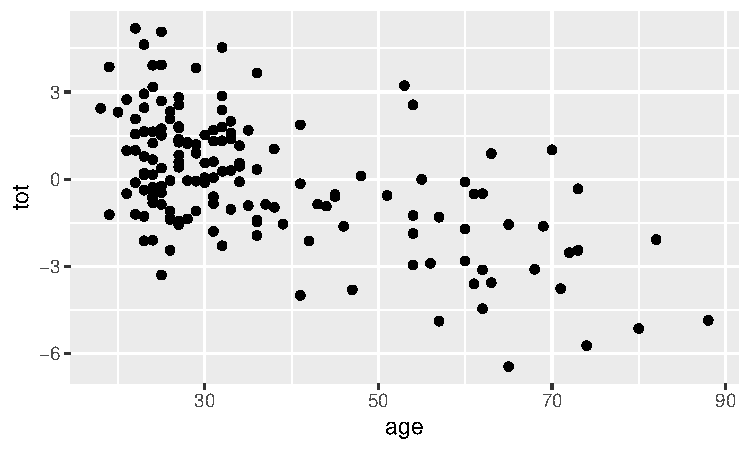
\includegraphics{hmk1Stat495F22_files/figure-latex/unnamed-chunk-5-1.pdf}

\begin{Shaded}
\begin{Highlighting}[]
\FunctionTok{summary}\NormalTok{(lm1)}
\end{Highlighting}
\end{Shaded}

\begin{verbatim}
## 
## Call:
## lm(formula = age ~ tot + totSq + totCu, data = kidney)
## 
## Residuals:
##    Min     1Q Median     3Q    Max 
## -27.69  -7.95  -2.19   4.86  39.66 
## 
## Coefficients:
##             Estimate Std. Error t value Pr(>|t|)    
## (Intercept) 33.75153    1.23179   27.40  < 2e-16 ***
## tot         -3.94479    0.79948   -4.93  2.1e-06 ***
## totSq        0.55736    0.15557    3.58  0.00046 ***
## totCu        0.00403    0.04498    0.09  0.92879    
## ---
## Signif. codes:  0 '***' 0.001 '**' 0.01 '*' 0.05 '.' 0.1 ' ' 1
## 
## Residual standard error: 12.6 on 153 degrees of freedom
## Multiple R-squared:  0.385,  Adjusted R-squared:  0.373 
## F-statistic: 31.9 on 3 and 153 DF,  p-value: 4.5e-16
\end{verbatim}

\begin{Shaded}
\begin{Highlighting}[]
\NormalTok{pred }\OtherTok{=} \FunctionTok{augment}\NormalTok{(lm1, }\AttributeTok{se\_fit =} \ConstantTok{TRUE}\NormalTok{) }\SpecialCharTok{\%\textgreater{}\%}
  \FunctionTok{filter}\NormalTok{(age}\SpecialCharTok{\%\%}\DecValTok{10} \SpecialCharTok{==} \DecValTok{0}\NormalTok{) }\SpecialCharTok{\%\textgreater{}\%}
  \FunctionTok{select}\NormalTok{(age, .fitted, .se.fit) }\SpecialCharTok{\%\textgreater{}\%}
  \FunctionTok{rename}\NormalTok{(}\StringTok{"Age"} \OtherTok{=}\NormalTok{ age, }\StringTok{"Estimates"} \OtherTok{=}\NormalTok{ .fitted, }\StringTok{"Standard Errors"} \OtherTok{=}\NormalTok{ .se.fit)}

\NormalTok{ pred }\SpecialCharTok{\%\textgreater{}\%}\NormalTok{ knitr}\SpecialCharTok{::}\FunctionTok{kable}\NormalTok{(}\AttributeTok{bookends =} \ConstantTok{TRUE}\NormalTok{)}
\end{Highlighting}
\end{Shaded}

\begin{longtable}[]{@{}rrr@{}}
\toprule()
Age & Estimates & Standard Errors \\
\midrule()
\endhead
20 & 27.6760 & 1.68969 \\
30 & 29.0573 & 1.51572 \\
30 & 31.7179 & 1.29991 \\
30 & 33.5557 & 1.23420 \\
30 & 34.2329 & 1.22953 \\
60 & 34.1516 & 1.22955 \\
60 & 49.1481 & 1.99318 \\
60 & 42.1650 & 1.61062 \\
70 & 30.3400 & 1.39696 \\
80 & 68.2063 & 4.07611 \\
\bottomrule()
\end{longtable}

\begin{Shaded}
\begin{Highlighting}[]
\CommentTok{\# Do you remember how to add powers to a regression? You can also use mutate. }
\CommentTok{\# Be sure you actually get a cubic regression! }
\CommentTok{\# The model must show the appropriate terms.}
\end{Highlighting}
\end{Shaded}

\begin{quote}
\begin{enumerate}
\def\labelenumi{(\alph{enumi})}
\setcounter{enumi}{1}
\tightlist
\item
  How do the results compare with those in Table 1.1?
\end{enumerate}
\end{quote}

SOLUTION:

\newpage

\hypertarget{casi-1.4---slightly-modified}{%
\subsection{CASI 1.4 - Slightly
Modified}\label{casi-1.4---slightly-modified}}

\begin{Shaded}
\begin{Highlighting}[]
\CommentTok{\# Load and format data}
\NormalTok{leukemia\_big }\OtherTok{\textless{}{-}} \FunctionTok{read.csv}\NormalTok{(}\StringTok{"http://web.stanford.edu/\textasciitilde{}hastie/CASI\_files/DATA/leukemia\_big.csv"}\NormalTok{)}
\CommentTok{\# says pictures from row 136}
\NormalTok{gene136 }\OtherTok{\textless{}{-}} \FunctionTok{t}\NormalTok{(leukemia\_big[}\DecValTok{136}\NormalTok{, ]) }\CommentTok{\#says pictures from row 136}
\CommentTok{\# Need to get ALL and AML tags in}
\NormalTok{type }\OtherTok{\textless{}{-}} \FunctionTok{c}\NormalTok{(}\FunctionTok{rep}\NormalTok{(}\StringTok{"ALL"}\NormalTok{, }\DecValTok{20}\NormalTok{), }\FunctionTok{rep}\NormalTok{(}\StringTok{"AML"}\NormalTok{, }\DecValTok{14}\NormalTok{), }\FunctionTok{rep}\NormalTok{(}\StringTok{"ALL"}\NormalTok{, }\DecValTok{27}\NormalTok{), }\FunctionTok{rep}\NormalTok{(}\StringTok{"AML"}\NormalTok{, }\DecValTok{11}\NormalTok{))}

\CommentTok{\# Set up dataset}
\NormalTok{leukemia }\OtherTok{\textless{}{-}} \FunctionTok{data.frame}\NormalTok{(gene136, type)}
\NormalTok{leukemia }\OtherTok{\textless{}{-}} \FunctionTok{rename}\NormalTok{(leukemia, }\AttributeTok{gene136 =}\NormalTok{ X136)}
\FunctionTok{favstats}\NormalTok{(}\SpecialCharTok{\textasciitilde{}}\NormalTok{ gene136 }\SpecialCharTok{|}\NormalTok{ type, }\AttributeTok{data =}\NormalTok{ leukemia)}
\end{Highlighting}
\end{Shaded}

\begin{verbatim}
##   type      min       Q1   median       Q3     max     mean       sd  n missing
## 1  ALL 0.210578 0.560344 0.732703 0.855127 1.63400 0.752479 0.275342 47       0
## 2  AML 0.324703 0.771426 0.967796 1.096250 1.42548 0.949973 0.243019 25       0
\end{verbatim}

We want to see if there is a significant difference in mean gene
expression for gene 136 for the ALL and AML groups.

\begin{quote}
\begin{enumerate}
\def\labelenumi{(\alph{enumi})}
\tightlist
\item
  Record the means of the ALL and AML groups for the gene 136 data
  available for reference.
\end{enumerate}
\end{quote}

SOLUTION: The mean of the ALL group for the gene 136 is 0.752 and the
mean of the AML group for the gene 136 is 0.950.

\begin{quote}
\begin{enumerate}
\def\labelenumi{(\alph{enumi})}
\setcounter{enumi}{1}
\tightlist
\item
  Perform 1000 nonparametric bootstrap replications for the mean of ALL
  for gene 136. Describe the distribution of the resulting means. You
  can perform the bootstrap in any way you see fit (the functions do and
  resample might prove useful).
\end{enumerate}
\end{quote}

\begin{Shaded}
\begin{Highlighting}[]
\NormalTok{leukemia\_ALL }\OtherTok{\textless{}{-}}\NormalTok{ leukemia }\SpecialCharTok{\%\textgreater{}\%}
  \FunctionTok{filter}\NormalTok{(type }\SpecialCharTok{==} \StringTok{"ALL"}\NormalTok{)}
  
\NormalTok{leukemia\_ALL}
\end{Highlighting}
\end{Shaded}

\begin{verbatim}
##         gene136 type
## ALL    0.918695  ALL
## ALL.1  1.634002  ALL
## ALL.2  0.459587  ALL
## ALL.3  0.637966  ALL
## ALL.4  0.344038  ALL
## ALL.5  0.861478  ALL
## ALL.6  0.513218  ALL
## ALL.7  0.979090  ALL
## ALL.8  0.210578  ALL
## ALL.9  0.801607  ALL
## ALL.10 0.600695  ALL
## ALL.11 0.361437  ALL
## ALL.12 1.046320  ALL
## ALL.13 0.969763  ALL
## ALL.14 0.487316  ALL
## ALL.15 0.497636  ALL
## ALL.16 1.101717  ALL
## ALL.17 0.856394  ALL
## ALL.18 0.661415  ALL
## ALL.19 0.817711  ALL
## ALL.20 0.567954  ALL
## ALL.21 0.846290  ALL
## ALL.22 0.883862  ALL
## ALL.23 0.723993  ALL
## ALL.24 0.732703  ALL
## ALL.25 0.782362  ALL
## ALL.26 0.543540  ALL
## ALL.27 0.832537  ALL
## ALL.28 0.552733  ALL
## ALL.29 0.732703  ALL
## ALL.30 0.551095  ALL
## ALL.31 0.821401  ALL
## ALL.32 0.641850  ALL
## ALL.33 0.720798  ALL
## ALL.34 0.583100  ALL
## ALL.35 0.765757  ALL
## ALL.36 0.526298  ALL
## ALL.37 1.466999  ALL
## ALL.38 0.544559  ALL
## ALL.39 0.572505  ALL
## ALL.40 1.362768  ALL
## ALL.41 0.853353  ALL
## ALL.42 0.813298  ALL
## ALL.43 0.853860  ALL
## ALL.44 0.568988  ALL
## ALL.45 0.693035  ALL
## ALL.46 1.067526  ALL
\end{verbatim}

\begin{Shaded}
\begin{Highlighting}[]
\NormalTok{boot }\OtherTok{\textless{}{-}} \FunctionTok{bootstrap}\NormalTok{(}\AttributeTok{data =}\NormalTok{ leukemia\_ALL, }\FunctionTok{mean}\NormalTok{(leukemia\_ALL}\SpecialCharTok{$}\NormalTok{gene136), }\AttributeTok{R =} \DecValTok{1000}\NormalTok{, }\AttributeTok{seed =} \DecValTok{0}\NormalTok{ )}

\CommentTok{\#resample(leukemia\_ALL, resampleFun = mean, replace = TRUE)}
\end{Highlighting}
\end{Shaded}

SOLUTION:

\begin{quote}
\begin{enumerate}
\def\labelenumi{(\alph{enumi})}
\setcounter{enumi}{2}
\tightlist
\item
  Repeat (b) for AML.
\end{enumerate}
\end{quote}

SOLUTION:

\begin{quote}
\begin{enumerate}
\def\labelenumi{(\alph{enumi})}
\setcounter{enumi}{3}
\tightlist
\item
  Suggest an inference. In other words, what do your results in (b) and
  (c) suggest about whether there is a difference in means for the ALL
  and AML groups for gene 136?
\end{enumerate}
\end{quote}

SOLUTION:

\begin{quote}
\begin{enumerate}
\def\labelenumi{(\alph{enumi})}
\setcounter{enumi}{4}
\tightlist
\item
  Brainstorm an alternative way to approach the problem via a
  randomization/permutation test. Describe what you would do in a way
  that someone else could code it up. (You do not need to actually code
  this up, but you can if you want to see what the result is.)
\end{enumerate}
\end{quote}

SOLUTION:

\newpage

\hypertarget{portfolio-reflection}{%
\subsection{Portfolio Reflection}\label{portfolio-reflection}}

Look at our portfolio review and in-class activities. In a separate word
or pdf document, in a few paragraphs, reflect on how the items in your
portfolio demonstrate:

\begin{itemize}
\tightlist
\item
  how your statistical analytical skills have developed over time
\item
  how your statistical writing skills have developed over time
\item
  skills you have a solid grasp of (such as R code or visuals or
  regression)
\item
  skills you would like to improve on
\end{itemize}

Then, set some goals for what you'd like to work on improving in future
statistical reports. (Yes, you brainstormed some before, this is asking
you to pick some to really focus on!)

Upload this portfolio reflection and goals document for future reports
to your portfolio folder in your personal class repo.

Given what you are asked to include, I expect the document to have at
least 3 paragraphs and contain at least 3 goals for future work.

\end{document}
